% Drawing 74/01-5 -- folder 74, batch 01, archive page 20 (PDF page 21).
% Transcription: Le bas de la page est couvert d'esquisses sans légende : colonnes et grilles $3\times 3$ de points (l'une entourée d'un cercle), un faisceau de segments croisés entre deux rangées de points, de petits polyèdres, deux triangles, et les inscriptions « $x\,y\,z\,x'y'z'$ » (avec une accolade), « $9\ 6\ 6\ 6$ », « $9\ 9\ 9$ » et « $40$ ». Dans la marge droite, quelques traits illisibles.
% Kind: page of sketches (point grids, polyhedra, numbers). Method 2 (schematic redraw from the facsimile). Status: partial.
% Notes: Bottom of the page, every stroke redrawn where it lies: three columns of three points, the middle one joined by a bold stroke (the middle point of the right column is a short stroke); a closed curve, notched at its upper right, around a 3x3 grid of points (two of them short dashes), with a short vertical stroke across its left side and three small marks above it; a bundle of ten crossed strokes between a row of four blots above and four below, drawn stroke for stroke (several start beside a blot rather than at it, and one stops halfway, as on the page); x y z x'y'z' with a bracket under x y z; a small polyhedron (pentagon outline, an inner vertex joined to four corners, and one diagonal); a second 3x3 grid; 9 6 6 6 with a bracket over 9 6, and 9 9 9; 40; two triangles one above the other (the lower one open at its apex); two isolated points; and a polyhedron with a pentagonal outline and inner edges, half hidden by an ink blot. The two ink stains, the illegible strokes in the right margin, the line « X = prod E_alpha » above and the page number are not drawn. Labels at \small, the figure drawn at 1.5 mm per unit so that they keep their places. Redrawn 2026-11-09 (issue 128); overlay check 2026-11-13 (issue 147). Second pass 2026-11-14 (issue 147, Claude claude-opus-5-5): every stroke and point re-read on 22 to 90 px/unit gridded crops of the 400 dpi colour scan and redrawn there (the circle, its grid and the left columns lay 1 to 2 units off, and the bundle was drawn as strokes between its end points). Rasterised by the session's previewer (not compiled: no TeX in the session) and laid over the crop: every stroke, point and label lies on its ink to within about 1 unit. Still differs: the inner edges of the last polyhedron under the ink blot are a reading (those visible beside the blot are drawn; what the blot covers is not). Not checked by a reader.
% Coordinates: 1 unit = 1.5 mm = 1/100 of the crop width (bbox in page fractions: [0.08, 0.6, 0.95, 0.88]).
% Redrawn by Claude (claude-opus-5-5), issue #73, 2026-11-09; not checked by a human; not compiled (no TeX in the session).
% Checked by Claude (claude-opus-5-5) 2026-11-13 (issue #147): overlaid on the 300 dpi colour facsimile; not compiled (no TeX in the session). Status: partial.
% Second pass by Claude (claude-opus-5-5) 2026-11-14 (issue #147): redrawn stroke by stroke from the 400 dpi colour facsimile, overlaid on a grid; not compiled (no TeX in the session). Status: partial.
% Rights: reproduces part of the work -- behind RENDER_TRANSCRIPTS, never published by itself.
\documentclass[tikz,border=3pt]{standalone}
\usepackage{amsmath,amssymb}
\usetikzlibrary{patterns,arrows.meta}
\tikzset{pencil/.style={black!45}, struck/.style={black!35}, mark/.style={circle,draw,inner sep=1.3pt}, pt/.style={circle,fill,inner sep=0.9pt}, opt/.style={circle,draw,fill=white,inner sep=1.1pt}}
\begin{document}
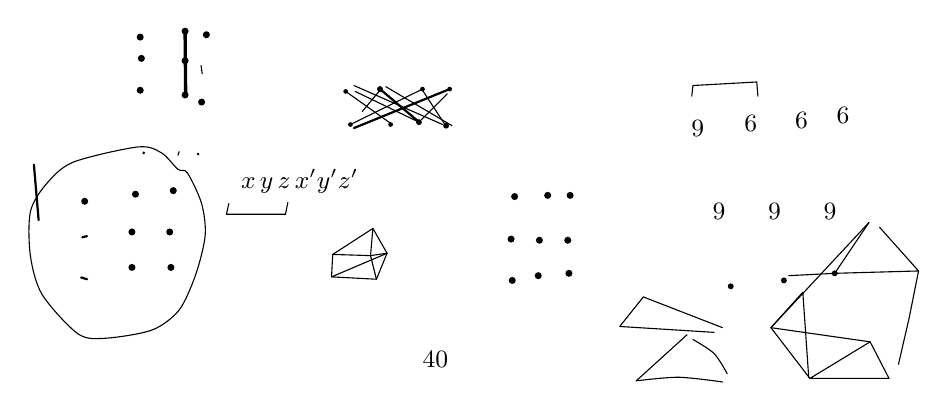
\begin{tikzpicture}[x=1.5mm,y=1.5mm,line cap=round,line join=round,font=\scriptsize]
% three columns of three points, the middle one joined by a bold stroke
\node[pt] at (18,-4.2) {};
\node[pt] at (18.1,-6) {};
\node[pt] at (18,-8.7) {};
\node[pt] at (21.8,-3.7) {};
\node[pt] at (21.8,-6.2) {};
\node[pt] at (21.8,-9.1) {};
\node[pt] at (23.6,-4) {};
\draw (23.15,-6.6) -- (23.25,-7.3);
\node[pt] at (23.2,-9.7) {};
\draw[very thick] (21.8,-3.7) -- (21.85,-9.1);
% closed curve round a 3 x 3 grid of points
\draw plot[smooth cycle, tension=0.5] coordinates {(17.8,-13.5) (12.3,-14.8) (10,-16.7) (8.7,-19) (8.7,-22.7) (9.7,-26) (12.7,-29.3) (15,-29.7) (19,-29) (21.3,-27.3) (22.7,-24.3) (23.5,-21) (23.2,-18.3) (22,-15.7) (21.2,-15.4) (19.8,-14)};
\draw[thick] (9,-15) -- (9.4,-19.7);
\node[pt] at (13.3,-18.1) {};
\node[pt] at (17.6,-17.5) {};
\node[pt] at (20.8,-17.2) {};
\draw[thick] (13.1,-21.15) -- (13.5,-21.05);
\node[pt] at (17.3,-20.7) {};
\node[pt] at (20.5,-20.7) {};
\draw[thick] (13,-24.55) -- (13.5,-24.7);
\node[pt] at (17.3,-23.7) {};
\node[pt] at (20.6,-23.7) {};
\fill (18.3,-14) circle[radius=0.12];
\draw (21.3,-13.9) -- (21.2,-14.2);
\fill (22.9,-14.1) circle[radius=0.12];
% the crossed bundle, stroke by stroke
\draw (35.4,-8.8) -- (39.2,-11.5);
\draw (36.1,-8.3) -- (43.6,-11.6);
\draw (36.2,-8.8) -- (41.6,-11.4);
\draw (38.3,-8.7) -- (36.8,-10.5);
\draw[thick] (38.3,-8.6) -- (41.5,-11.3);
\draw (38.8,-8.4) -- (44.4,-11.7);
\draw (41.9,-8.6) -- (35.8,-11.6);
\draw (41.9,-8.7) -- (43.8,-11.6);
\draw[thick] (44.2,-8.6) -- (36.1,-11.9);
\draw (44,-9) -- (41.8,-11.2);
\fill (35.4,-8.8) circle[radius=0.2];
\fill (38.3,-8.6) circle[radius=0.25];
\fill (41.9,-8.6) circle[radius=0.2];
\fill (44.2,-8.6) circle[radius=0.2];
\fill (35.8,-11.6) circle[radius=0.2];
\fill (39.2,-11.6) circle[radius=0.2];
\fill (41.6,-11.4) circle[radius=0.25];
\fill (43.9,-11.7) circle[radius=0.25];
% x y z x' y' z' with a bracket under x y z
\node[inner sep=1pt] at (31.5,-16.4) {\small $x\,y\,z\,x'y'z'$};
\draw (25.5,-18.3) -- (25.3,-19.2) -- (30.3,-19.2) -- (30.5,-18.2);
% small polyhedron
\draw (34.3,-22.6) -- (37.7,-20.4) -- (38.9,-22.5) -- (38,-24.7) -- (34.2,-24.5) -- cycle;
\draw (34.3,-22.6) -- (37.5,-22.7) -- (38.9,-22.5);
\draw (37.5,-22.7) -- (37.7,-20.4);
\draw (37.5,-22.7) -- (38,-24.7);
\draw (34.2,-24.5) -- (38.9,-22.5);
% 3 x 3 points
\node[pt] at (49.7,-17.7) {};
\node[pt] at (52.5,-17.6) {};
\node[pt] at (54.4,-17.6) {};
\node[pt] at (49.4,-21.3) {};
\node[pt] at (51.8,-21.4) {};
\node[pt] at (54.2,-21.4) {};
\node[pt] at (49.5,-24.8) {};
\node[pt] at (51.7,-24.4) {};
\node[pt] at (54.3,-24.2) {};
% numbers
\draw (64.7,-9.2) -- (64.8,-8.3) -- (70.2,-8) -- (70.3,-9.2);
\node[inner sep=1pt] at (65.2,-11.9) {\small $9$};
\node[inner sep=1pt] at (69.7,-11.5) {\small $6$};
\node[inner sep=1pt] at (74,-11.3) {\small $6$};
\node[inner sep=1pt] at (77.5,-10.8) {\small $6$};
\node[inner sep=1pt] at (67,-19) {\small $9$};
\node[inner sep=1pt] at (71.7,-19) {\small $9$};
\node[inner sep=1pt] at (76.4,-19) {\small $9$};
\node[inner sep=1pt] at (43,-31.5) {\small $40$};
% two triangles
\draw (60.6,-26.2) -- (67.3,-28.8);
\draw (60.6,-26.2) -- (58.6,-28.7) -- (66.6,-29.2);
\draw (64.3,-29.4) -- (60,-33.3);
\draw plot[smooth] coordinates {(60,-33.3) (63.6,-33) (67.3,-33.4)};
\draw plot[smooth] coordinates {(64.8,-29.8) (66.6,-31) (67.7,-32.7)};
\fill (68,-25.3) circle[radius=0.25];
\fill (72.5,-24.8) circle[radius=0.25];
% polyhedron under the ink blot
\draw (71.4,-28.8) -- (79.7,-19.9);
\draw (79.7,-19.9) -- (76.8,-24.2);
\draw (72.9,-24.4) -- (76.8,-24.2) -- (83.9,-24);
\draw (80.6,-20.3) -- (83.9,-24) -- (83.1,-28) -- (82.2,-31.9);
\draw (71.4,-28.8) -- (74.7,-33.1) -- (81.4,-33.1) -- (79.8,-30) -- (74.7,-33.1);
\draw (71.4,-28.8) -- (79.8,-30);
\draw (71.4,-28.8) -- (74.1,-25.8) -- (74.6,-33);
\fill (76.8,-24.2) circle[radius=0.25];
\end{tikzpicture}
\end{document}
